\section{Python Decision Making}
Pengambilan keputusan adalah antisipasi kondisi yang terjadi saat pelaksanaan program dan menentukan tindakan yang dilakukan sesuai kondisi. 
Struktur keputusan mengevaluasi banyak ekspresi yang menghasilkan TRUE atau FALSE sebagai hasil.   Anda perlu menentukan tindakan mana yang harus diambil dan pernyataan mana yang akan dijalankan jika hasilnya BENAR atau SALAH sebaliknya. 
Berikut adalah bentuk umum dari struktur pengambilan keputusan yang khas atau khusus yang ditemukan di sebagian besar bahasa pemrograman
\ref{diagramstruktur}.
\begin{figure}[ht]
    \centerline{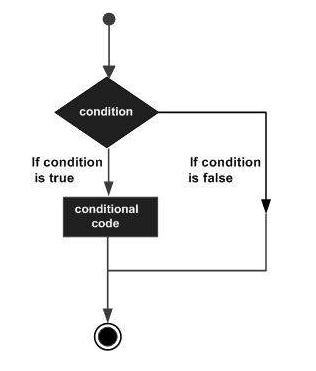
\includegraphics[width=0.25\textwidth]{figures/struktur}}
    \caption{struktur pada python}
    \label{diagramstruktur}
    \end{figure}
Bahasa pemrograman Python menyediakan jenis dan juga laporan pengambilan keputusan. Berikut ini adalah penjelasan tentang pernyataan dan deskripsinya :
\begin{enumerate}
\item
if statements : sebuah if statement terdiri dari ekspresi boolean diikuti oleh satu atau lebih pernyataan. 
\item
if...else statements : sebuah if statement dapat diikuti oleh opsinal else statement, yang mengeksekusi ketika ekspresi boolean adalah palsu. 
\item
nested if statements : anda dapat menggunakan satu if atau else if pernyataan di dalam lain if atau else if statements. 
\end{enumerate}
Decision making atau Pemilihan keputusan pada python sangat penting untuk pemrograman komputer. Akan ada banyak situasi saat Anda diberi dua pilihan atau lebih dan Anda harus memilih opsi berdasarkan kondisi yang diberikan. Misalnya,
\begin{enumerate} 
\item
Seorang murid dengan nilai lebih dari 90 disebut siswa pintar 
\item
Seorang murid dengan nilai dibawah 90 dan diatas 30 disebut Siswa Standard 
\item
Seorang murid dengan nilai dibawah 30 disebut siswa bodoh 
\end{enumerate}

Umumnya juga, decision making dalam bahasa pemrograman yang sering digunakan adalah :
\begin{enumerate}
\item
if...else statement : berguna saat kita harus mengambil keputusan dari dua pilihan. Misalnya, jika seorang siswa mendapatkan nilai lebih dari angka 95, maka siswa itu pintar, jika tidak, situasi seperti itu dapat dikodekan. 
\item
if...elseif...else statement : merupakan optional dari if...else statement, yang sangat berguna untuk menentukan berbagai kondisi yang lebih dari 2. 
\item
switch statement : merupakan alternative dari if statement. Setiap nilai disebut case, dan variabel yang dicek untuk setiap switch case. 
\end{enumerate}

F...ELIF...ELSE statement sama seperti IF...ELSEIF...ELSE pada bahasa pemrograman Java, yaitu digunakan menyeleksi beberapa ekspresi (lebih dari satu), apabila eskpresi1 pertama bernilai true, maka akan dijalankan statement1, jika ekspresi2 kedua bernilai true, maka akan dijalankan statement2, dan seterusnya.

Dari contoh diatas, pertanyaannya adalah bagaimana cara menulis kode pemrograman untuk menangani situasi seperti itu. Hampir semua bahasa pemrograman memberikan pernyataan kondisional diatas berdasarkan diagram decision di bawah. 
\begin{figure}[ht]
	    \centerline{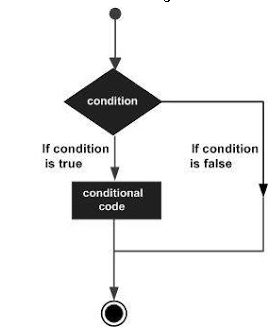
\includegraphics[width=0.25\textwidth]{figures/diagram_decision}}
	    \caption{diagram decision}
	    \label{diagramdecisionmaking}
	    \end{figure} 

Mari kita membuat sebuah program C dengan bantuan jika pernyataan kondisional untuk mengubah situasi yang diberikan di atas menjadi kode pemrograman:  
\begin{verbatim}
#include <stdio.h>
 
main() {
   int x = 45;
   if( x > 95) {
      printf( "siswa pintar");
   }
   if( x < 30) {
      printf( "siswa bodoh");
   }
   if( x < 95 && x > 30 ) {
      printf( "Siswa Standard");
   }
}
\end{verbatim}
Outputnya adalah Siswa Standard

Bahasa pemrograman Python mengasumsikan nilai   non-nol   dan   non-nullsebagai TRUE, dan jika itu adalah   nol   atau   nol   , maka diasumsikan sebagai nilai FALSE. 
Bahasa pemrograman Python menyediakan jenis pernyataan pengambilan keputusan berikut. 

 
Mari kita membahas setiap keputusan secara singkat  

 
Setelah tutorial mengenai  
\subsection{variable dan operator}
pada bahasa pemrograman python akan membahas mengenai percabangan/pengambilan keputusan. Percabangan atau pengambilan keputusan adalah pengkondisian yang terjadi ketika aplikasi berjalan, kemudian ada aksi-aksi tertentu atau kondisi tertentu sehingga aplikasi harus bereaksi terhadap hal itu. Atau dalam bahasa pemrograman umum dikenal dengan IF, THEN, ELSE sebagai contoh pengaplikasian dari pengambilan keputusan ini. 

if statements
Sebuah if statement terdiri dari ekspresi boolean diikuti oleh satu atau lebih pernyataan.
 
Pada pembahasan python decisiom makaing ini, kami menggunakan perangkat raspberry pi 2 dengan sistem operasi rasbian jessie. Sangat ringan dan tentunya python secara default ada di dalamnya. Kebetulan dalam tulisan ini masih menggunakan python versi 2, meskipun ada python versi 3 juga. 

 
Python core tidak menyediakan   \" switch  \"  atau   " case  \"  seperti bahasa pemrograman lain. Tapi kita bisa menggunakan statemen if, elif yang bisa menggantikan   \" switch  \"  atau   \" case  \" . 

 
Di bawah ini merupakan tipe-tipe percabangan yang disediakan oleh python. 

 
IF : Mengandung ekspresi boolean dan diikuti oleh satu atau banyak statemen 

 
IF ELSE : IF bisa diikuti oleh optional statemen yaitu ELSE, yang akan dieksekusi ketika ekspresi boolean bernilai FALSE 

 
NESTED IF atau IF bersarang :~ Kita bisa menggunakan IF, ELSE IF di dalam IF, ELSE IF lainnya 

 
Contoh dalam python untuk IF :  

 
varAngka1 = 123 

 
varAngka2 = 0 

 
if varAngka1: 

 
                                               print "Nilai : TRUE" 

 
                                                print varAngka1 

 
if varAngka2: 

 
                                               print "Nilai : TRUE" 

 
print varAngka2{\fontsize{14pt}{14pt}\selectfont     \\} 

 
\begin{verbatim}
#/usr/bin/python
a = raw_input("Masukkan Angka = ")
b = int(a)
if (b%2==0):
        print "Genap"
else:
        print "Ganjil"
\end{verbatim}

Contoh untuk IF ELIF ELSE, di python sintak ini bisa ditulis dengan lebih singkat yaitu elif :  

 
varAngka = 123 
 
    
 
if varAngka==200: 

 
                           print "Nilai : TRUE" 

 
                           print varAngka 

 
elif varAngka==123: 

 
                           print "Nilai : TRUE" 

 
                           print varAngka 

 
else: 

 
                           print "Nilai : FALSE" 

 
                           print varAngka 

 
Contoh untuk NESTED IF :  

\begin{verbatim}
varAngka = 89 
 
    
 
if varAngka<100: 

 
                       print \"Nilai : TRUE\" 

 
                       print varAngka 

 
                       if varAngka > 80: 

 
                                                print \"Nilai : A\" 

 
                       elif varAngka > 60: 

 
                                                print \"Nilai : B\" 

 
                       elif varAngka > 40: 

 
                                              print \"Nilai : C\" 

 
                       elif varAngka > 20: 

 
                                             print \"Nilai : D\" 

 
                        $else: 

 
                                            \ print \"Nilai : E\" 

 
else: 

                        print \"Nilai : FALSE\" 

 
                        print varAngka 
  end{verbatim}


Contoh lain pada NESTED IF dengan kondisi pilihan lebih dari satu. Seperti menentukan game yang sangat disukai : 
\vspace{12}
 
Begin{verbatim}
#/usr/bin/python
pilihan=2
if pilihan==1:
        print "DOTA 2"
else:
        if pilihan==2:
		print "GTA V Online"
	else:
		print "Semua Game"
end{verbatim}

Perintah seperti diatas itu adalah NESTED IF yaitu terdapat IF di dalam IF. 

 
Statemen IF juga bisa ditulis dalam 1 baris saja, misalnya seperti ini :  

 
if varAngka1: print \"Nilai : TRUE\" 

 
Dari sintak percabangan sudah bisa kita lihat perbedaan di antara python dengan menggunakan bahasa pemrograman yang lain. Sintak ditulis dengan lebih ringkas dibanding dengan yang lain. Percabangan atau pengkondisian ini adalah hal dasar dalam pemrograman pada umumnya, kita pasti akan menggunakannya. Pada tulisan yang akan dibuat selanjutnya saya akan menulis mengenai perulangan atau looping dalam python. 

 
Suite pernyataan tunggal 

 
Jika rangkaian   klausa   jika   hanya terdiri dari satu baris, itu mungkin sama pada baris perintah sebagai pernyataan header. 

 
Berikut adalah contoh   klausa   satu baris jika   - 


 
var = 100 

 
if ( var~ == 100 ) : print "Value of expression is 100" 

 
print "Good bye!" 

 
Bila kode diatas dieksekusi, maka menghasilkan hasil sebagai berikut - 

 
Value of expression is 100 

 
Good bye! \hspace*{1.31in}  
 

 
Pengambilan keputusan (kondisi if) digunakan untuk mengantisipasi kondisi yang terjadi saat jalanya program dan menentukan tindakan apa yang akan diambil sesuai dengan kondisi. 
 

 
Pada python ada beberapa statement atau kondisi diantaranya adalah   if,   else   dan   elif   Kondisi   if   digunakan untuk mengeksekusi kode jika kondisi bernilai benar. 
 

 
Jika kondisi bernilai salah maka statement atau kondisi if tidak akan di-eksekusi. 
 

Dibawah ini adalah contoh penggunaan kondisi if pada Python 
 

Dari contoh diatas, jika program dijalankan maka akan mencetak string \"Selamat Anda Lulus Ujian\" sebanyak 1 kali yaitu pada if pertama. Di if kedua statement bernilai salah, jadi perintah   print(\"Selamat Anda Lulus\")   tidak akan dieksekusi. 
 

Selanjutnya Anda bisa mempelajari kondisi if else 

 
Pengambilan keputusan (kondisi if else) tidak hanya digunakan untuk menentukan tindakan apa yang akan diambil sesuai dengan kondisi, tetapi juga digunakan untuk menentukan tindakan apa yang akan diambil atau dijalankan jika kondisi tidak sesuai.

 
 
Pada python ada beberapa statement atau kondisi diantaranya adalah   if,   else   dan   elif   Kondisi   if   digunakan untuk mengeksekusi kode jika kondisi bernilai benar.

 
 
Kondisi if else adalah kondisi dimana jika pernyataan benar (true) maka kode dalam if akan dieksekusi, tetapi jika bernilai salah (false) maka akan mengeksekusi kode di dalam else.

 
 
Dibawah ini adalah contoh penggunaan kondisi if else pada Python 

 
Kondisi if else adalah jika kondisi bernilai TRUE maka akan dieksekusi pada if, tetapi jika bernilai FALSE maka akan dieksekusi kode pada else 
 

nilai = 3
 
 
Jika pernyataan pada if bernilai TRUE maka if akan dieksekusi, tetapi jika FALSE kode pada else yang akan dieksekusi.
 
 
if(nilai > 7):
        
 
 print(\"Selamat Anda Lulus\")
 
 
else:
 
 
        print(\"Maaf Anda Tidak Lulus\") 
 


Pada contoh diatas, jika program dijalankan maka akan mencetak string \"Maaf Anda Tidak Lulus\" karena pernyataan pada if bernilai FALSE 
 

Selanjutnya kita akan mempelajari per-kondisi an pada python yang terakhir yaitu \"Elif\"    

 
Pengambilan keputusan (kondisi if elif) merupakan lanjutan atau percabangan logika dari \"kondisi if\". Dengan elif kita bisa membuat kode program yang akan menyeleksi beberapa kemungkinan yang bisa terjadi. Hampir sama dengan kondisi \"else\", bedanya kondisi \"elif\" bisa banyak dan tidak hanya satu.   

Dibawah ini adalah contoh penggunaan kondisi elif pada Python 

 
Contoh penggunaan kondisi elif 

 
hari   \_  ini = \"Minggu\" 
 


if(hari   \_  ini == \"Senin\"): 
 

        print(\"Saya akan kuliah\") 
 

elif(hari   \_  ini == \"Selasa\"): 
 

        print(\"Saya akan kuliah\") 
 

elif(hari   \_  ini == \"Rabu\"): 
 

        print(\"Saya akan kuliah\") 
 

elif(hari   \_  ini == \"Kamis\"): 
 

        print(\"Saya akan kuliah\") 
 

elif(hari   \_  ini == \"Jumat\"): 
 

 $  $  $  $ print("Saya akan kuliah") 
 

elif(hari $  \_  $ini == "Sabtu"): 
 

 $  $  $  $ print("Saya akan kuliah") 
 

elif(hari $  \_  $ini == "Minggu"): 
 

 $  $  $  $ print("Saya akan libur") 
 


Pada contoh diatas, jika program dijalankan maka akan mencetak   
\"Saya akan libur\". 
 
    Pernyataan tersebut digunakan untuk pengambilan keputusan dalam python berupa if, pernyataan tersebut memiliki format lengkap  yang dapat dilihat sebagai berikut : 

 
\begin{enumerate}
\item
if kondisi   \_  1: 

 
~~~~~~ pernyataan   \_  pernyataan   \_  1 

 
\item
elif kondisi   \_  2: 

 
~~~~~~ pernyataan   \_  pernyataan   \_  2 

 
\item
elif kondisi   \_  3: 

 
~~~~~~ pernyataan   \_  pernyataan   \_  3 

 
\item
else kondisi   \_  n: 

 
~~~~~~ pernyataan   \_  pernyataan-n 

 
~~~~~~  
 
\item
if kondisi   \_  1,elif kondisi   \_  2,elif kondisi   \_  3,else kondisi   \_  n 

 
~~~~berupa~suatu ekspresi yang menghasilkan nilai logika (benar atau salah)    
 
~~~  
\end{enumerated}
 
Contoh Code yang dijalankan pada modus interaktif 


\begin{verbatim}
  x = 5 

 
~ y = 100 

 
~~~ terbesar = x 

 
~~ if terbesar < y: 

 
terbesar = y 

~~~ terbesar = 100  

\end{verbatim}
 
~~~  

 
  Python tidak menggunakan  \{   \}  untuk menyertakan blok kode untuk penggunaan if or loop or fungsi yang lainnya. Sebaliknya, python menggunakan titik dua (:) dan indentasi atau spasi untuk pernyataan  kelompok. Tes  boolean untuk if tidak perlu dalam tanda kurung (perbedaan besar dari C++ atau Java), dan dapat memiliki *elif* dan *else*. 
 

            Nilai apapun dapat digunakan sebagai if-test.
			pada   \" nol  \"  nilai-nilai semua dihitung sebagai false:Tidak ada,0,string kosong,list kosong, dictionary kosong.
			Ada juga tipe Boolean dengan dua nilai: True dan False (jika dikonversi ke int, ini adalah 1 dan 0). 
			Python memiliki operasi perbandingan yang biasa: \verb| ==, =, <, <=,>,> =| 
			Tidak seperti Java dan C.Operator boolean bisa juga di eja seperti * and *, * or *, * not * (Python tidak menggunakan gaya C). 

 
~~~~matakuliah = 'matematika'   matematika,fisika 
 
~~  
 
 nilai = 70 100,80,50 

 
~~~ if nilai >=100 or nilai>=80 : 

 
~~~~~~ if matakuliah == 'matematika': 

 
~~~~~~~~~ print 'anda mendapat nilai A dalam mata kuliah matematika' 

 
~~~ elif matakuliah == 'fisika': 

 
~~~~~~ print 'anda mendapat nilai A dalam mata kuliah Fisika' 

 
~~~ elif nilai >=70 and matakuliah=='matematika': 


 
~~~~~~ print 'anda mendapat nilai B dalam mata kuliah matematika' 

 
~~~ elif nilai >=70 and matakuliah=='fisika': 

 
~~~~~~ print 'anda mendapat nilai B dalam mata kuliah fisika' 

 
~~~ else: 

 
~~~~~~ print 'nilai dan~matakuliah~tidak~ada'~~~     

 
Seperti halnya bahasa pemrograman yang lain, tentu python juga mempunyai perintah untuk pengambilan suatu keputusan terhadap kondisi tertentu, yang disebut percabangan. Percabangan pada bahasa pemrograman python menggunakan perintah if, ya sama dengan bahasa pemrograman yang lain. Bagaimana cara menggunakan perintah if ini dalam bahasa pemrograman python? berikut adaah cara penggunaan percabangan if yang tepat
 

Cara penulisan dari perintah if secara garis besar adalah seperti berikut: 
 


if <kondisi 1>: 
 

   <perintah yang dijalankan 1> 
 

elif <kondisi 2>: 
 

<perintah yang dijalankan 2> 
 

else:
   <perintah yang dijalankan 3> 
 


Perintah-perintah yang dipergunakan antara lain 
 

If dan If bersarang 
 

Elif (singkatan dari: else if) dan 
 

else.
 
 

IF Bersarang 
 

Adapun tanda titik dua diletakan setelah kondisi, sedangkan untuk perintah yang dijalankan jika kondisi if terpenuhi diberi tab atau 4 spasi pada depannya untuk menandakan bahwa perintah tersebut berada didalam if, contoh dalam source code. Misal kita ingin menentukan angka genap atau ganjil: 
 

angka = 7 
 

if angka    \%   2 == 0: 
 

        print 'genap' 
 

else:
   print 'ganjil' 
 

 Dari perintah diatas akan menghasilkan nilai yang diprint adalah 'ganjil'. Tanda  $  \%  $ (persen) disini merupakan operator untuk modulus, yaitu sisa bagi. Adapun jalannya dari program diatas adalah, jika angka dalam hal ini nilainya 7 jika di modulus dengan 2, menyisahkan nilai nol maka data yang diprint adalah genap, jika tidak menyisahkan nilai nol maka data yang diprint adalah ganjil. 
 

Bagaimana halnya dengan kondisi yang lebih dari satu. Misal kita ingin menentukan game yang kita sukai: 
 

pilihan = 2 
 

if pilihan == 1: 
 

        print 'DOTA2' 
 

else:
        if pilihan == 2: 
 

                print 'GTA V Online' 
 

        else: 
 

                print 'Semua Game' 
 

Perintah diatas merupakan if bersarang yaitu terdapat if didalam if, dapat juga dituliskan dengan perintah dibawah ini dengan menggunakan elif: 
 


Elif 
 

Merupakan suatu pemilihan kondisi dimana dalam kondisi tersebut, terdapat lagi kondisi lain
Contoh kodingnya : 
 

Program Kategori Berat hewan qurban 
 

pilihan = 300 
 

if pilihan > 300: 
 

        print 'Sapi boleh diqurban' 
 

elif pilihan <    300 : 
 

        print 'Sapi belum boleh diqurban' 
 

else: 
 

        print ‘Rawat dulu sapinya yang benar' 
 

Mana yang terbaik dari kedua cara penulisan kondisi if yang lebih dari satu diatas itu tentunya sesuai dengan kebutuhan kita masing-masing dalam membuat suatu aplikasi. Dalam if pun kita bisa membuat dua atau lebih persyaratan dalam kondisi if 
 


Else 
 

contohnya:
angka = 2 
 

if angka <= 10 and angka >= 1 : 
 

        print 'angka diantara 1 dan 10' 
 

else: 
 

        print 'angka diluar jangkauan' 

 
Percabangan Pada Bahasa Pemrograman Python. 

 
Seperti halnya bahasa pemrograman yang lain, tentu python juga mempunyai perintah untuk pengambilan suatu keputusan terhadap kondisi tertentu, yang disebut percabangan. Percabangan pada bahasa pemrograman python menggunakan perintah   if, ya sama dengan bahasa pemrograman yang lain. Bagaimana cara menggunakan perintah   if   ini dalam bahasa pemrograman python? Yuk mari kita sama-sama melihat cara penggunaan perintah   if   ini. 

 
Cara penulisan dari perintah if secara garis besar adalah seperti berikut: 
 
if <kondisi 1>: 

 
~~~ <perintah yang dijalankan 1> 

 
elif <kondisi 2>: 

 
~~~ <perintah yang dijalankan 2> 

 
else: 

 
~~~ <perintah yang dijalankan 3> 

 
Perintah-perintah yang dipergunakan antara lain   if,   elif   (singkatan dari:   else if) dan   else. Adapun tanda titik dua diletakan setelah kondisi, sedangkan untuk perintah yang dijalankan jika kondisi if terpenuhi diberi   tab   atau   4 spasi   pada depannya untuk menandakan bahwa perintah tersebut berada didalam if, contoh dalam source code. Misal kita ingin menentukan angka genap atau ganjil: 

 
angka = 7 

 
if angka    \%   2 == 0: 

 
~~~ print 'genap' 

 
else: 

 
~~~ print 'ganjil' 

 
Dari perintah diatas akan menghasilkan nilai yang diprint adalah 'ganjil'. Tanda      \%     (persen) disini merupakan operator untuk modulus, yaitu sisa bagi. Adapun jalannya dari program diatas adalah, jika angka dalam hal ini nilainya 7 jika di modulus dengan 2, menyisahkan nilai nol maka data yang diprint adalah genap, jika tidak menyisahkan nilai nol maka data yang diprint adalah ganjil. 

 
Bagaimana halnya dengan kondisi yang lebih dari satu. Misal kita ingin menentukan buah yang kita sukai: 

 
pilihan = 2 

 
if pilihan == 1: 

 
~~~ print 'buah durian' 

 
else: 

 
~~~ if pilihan == 2: 

 
~~~~~~~ print 'buah mangga' 

 
~~~ else: 

 
~~~~~~~ print 'semua buah' 

 
Perintah diatas merupakan if bersarang yaitu terdapat if didalam if, dapat juga dituliskan dengan perintah dibawah ini dengan menggunakan $  $elif: 

 
pilihan = 2 

 
if pilihan == 1: 

 
~~~ print 'buah durian' 

 
elif pilihan == 2: 

 
~~~ print 'buah mangga' 

 
else: 

 
~~~ print 'semua buah' 

 
Mana yang terbaik dari kedua cara penulisan kondisi if yang lebih dari satu diatas itu tentunya sesuai dengan kebutuhan kita masing-masing dalam membuat suatu aplikasi, seperti kata orang, banyak jalan menuju roma begitu juga dengan pemrograman, banyak jalan untuk menuliskan suatu perintah untuk menghasilkan hasil tertentu... :) 

 
Dalam if pun kita bisa membuat dua atau lebih persyaratan dalam kondisi   if   contohnya: 

 
\begin{verbatim}
angka = 2  
if angka <= 10 and angka >= 1 : 
~~~ print 'angka diantara 1 dan 10' 
else:  
~~~ print 'angka diluar jangkauan' 
\end{verbatim}



